\setbeamertemplate{navigation symbols}{}
\setbeamercolor{structure}{fg=uni-blue} % itemize, enumerate, etc
\setbeamercolor{normal text}{fg=uni-black}

\setbeamercolor{section in toc}{fg=uni-blue} % TOC sections
\setbeamercolor{subsection in toc}{fg=uni-black} % TOC sections

\setbeamertemplate{subsection  in toc}[square]
\setbeamertemplate{section in toc}[circle]

\setbeamerfont{section number projected}{size=\large}
\setbeamercolor{section number projected}{bg=uni-blue,fg=white}
\setbeamercolor{subsection number projected}{bg=uni-black,fg=white}

% Universal background except title
\usebackgroundtemplate{%
	
\includegraphics[width=\paperwidth,height=\paperheight]{images/otherbackground.pdf}} 

%----------------------------------------------------------------------------------------
%	FOOTER THEME
%----------------------------------------------------------------------------------------

\setbeamertemplate{footline}[text line]{%
		
	\setbeamercolor{footline}{bg=,fg=uni-blue}	
	
	\begin{beamercolorbox}[sep=0.3cm,ht=2.6em,wd=\paperwidth]{footline}
		
		\vbox{}\vskip-2ex%
		\hspace{0.0cm}
		\insertshortauthor
		\hfill
		\fontfamily{phv}\fontseries{bc}\selectfont\bfseries 
		\insertframenumber
		\hfill
		\vskip-0.8ex%
	\end{beamercolorbox}
	
}

%----------------------------------------------------------------------------------------
%	ITEMIZE CIRCLE
%----------------------------------------------------------------------------------------

\setbeamertemplate{itemize items}{
	
\begin{tikzpicture}
	\node[circle, draw, semithick, inner sep=0pt, minimum size=4pt] (1) at (0,0) {};
	\end{tikzpicture}
}

%----------------------------------------------------------------------------------------
%	TITLE PAGE
%----------------------------------------------------------------------------------------

\setbeamertemplate{title page}{%

	\begin{tikzpicture}[remember picture,overlay]
	
	% Uni logo
	\node[inner sep=0pt] (logo) at (1.1, 3)
	{
\includegraphics[width=.3\textwidth]{images/logo.pdf}};
	
	% Uni pic
	\node[inner sep=0pt] (logo) at (9.175, 1.62)
	{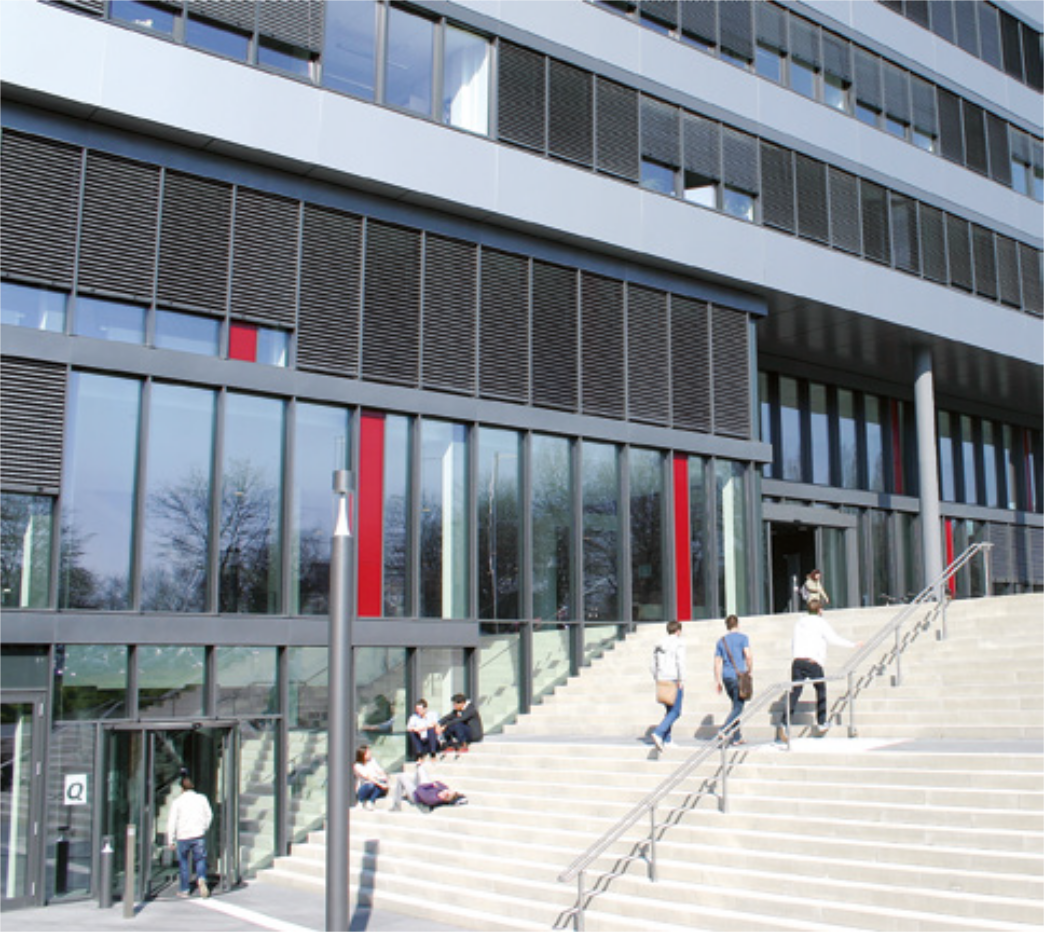
\includegraphics[width=.485\textwidth]{images/unibuilding.png}};
	

	\node[inner sep=0pt] (tit) at (4.40, -2.7)
	{
		\begin{minipage}[t]{1.0\linewidth} 
		\setbeamercolor{title}{bg=\upbcolor,fg=white}	
		
		\begin{minipage}[t]{1.0\linewidth} 
		\setbeamercolor{title}{bg=,fg=uni-blue}	
		\begin{beamercolorbox}[sep=2pt,left]{title}
		{\hspace{4pt}{\vspace{0.1cm}\fontsize{10}{16}\fontfamily{phv}\fontseries{bc}\selectfont\bfseries\insertinstitute}}
		\end{beamercolorbox}
		
		\end{minipage}  	
		
		\begin{minipage}{1.0\linewidth} 
		
		
		\begin{beamercolorbox}[sep=8pt,left]{title}
		
		{\lenitem{\fontsize{\upbtitlesize}{\upbtitlelinespace}\fontfamily{phv}\fontseries{mc}\selectfont\bfseries\color{white}\raggedright\inserttitle}}%
		
		\end{beamercolorbox}
		
		\end{minipage}  	
		
		\ifx\insertsubtitle\@empty%
		\else%
		{		\begin{minipage}[t]{0.9\linewidth} 
			\setbeamercolor{title}{bg=,fg=uni-blue}	
			\begin{beamercolorbox}[sep=4pt,left]{subtitle}
			{\hspace{4pt}\vspace{0.2cm}{\fontsize{10}{16}\fontfamily{phv}\fontseries{bc}\selectfont\bfseries \insertsubtitle}}
			\end{beamercolorbox}
			\end{minipage}  	
		}
		\fi%   			
		
		\end{minipage}  		
		
	};
	
	\end{tikzpicture}	
	
}

%----------------------------------------------------------------------------------------
%	FRAME TITLE THEME
%----------------------------------------------------------------------------------------

\setbeamertemplate{frametitle}
{
	\nointerlineskip
	
	\fontfamily{phv}\fontseries{bc}\selectfont\bfseries 
	\setbeamercolor{frametitle}{bg=,fg=\upbcolor}	
	
	\begin{beamercolorbox}[sep=0.3cm,ht=5.3em,wd=\paperwidth]{frametitle}
		\vbox{}\vskip-2ex%
		\hspace{0.05cm}
		
\includegraphics[width=1.8cm]{images/logo}
		\hfill
		\vskip1.2ex%
		\vspace{0.1cm}
		\hspace{0.0cm}
		\insertframetitle
	\end{beamercolorbox}
	\vspace{-0.4cm}
	
}
